\subsubsection{Support Vector Machines (SVM) Analysis}
\label{subsubsec:discussion-svm}

% SVMs performed well on both the hepatitis and the mushroom datasets,
% achieving peak accuracy and F1 scores which match the best results from KNN.

A key advantage of the SVM over KNN is that SVMs are much faster during consultation time. As seen in \autoref{fig:model_comparison_mushroom},
SVMs tend to have much lower test times than KNN. This is expecially noticable for large datasets like the mushroom dataset.

\begin{figure}
    \centering
    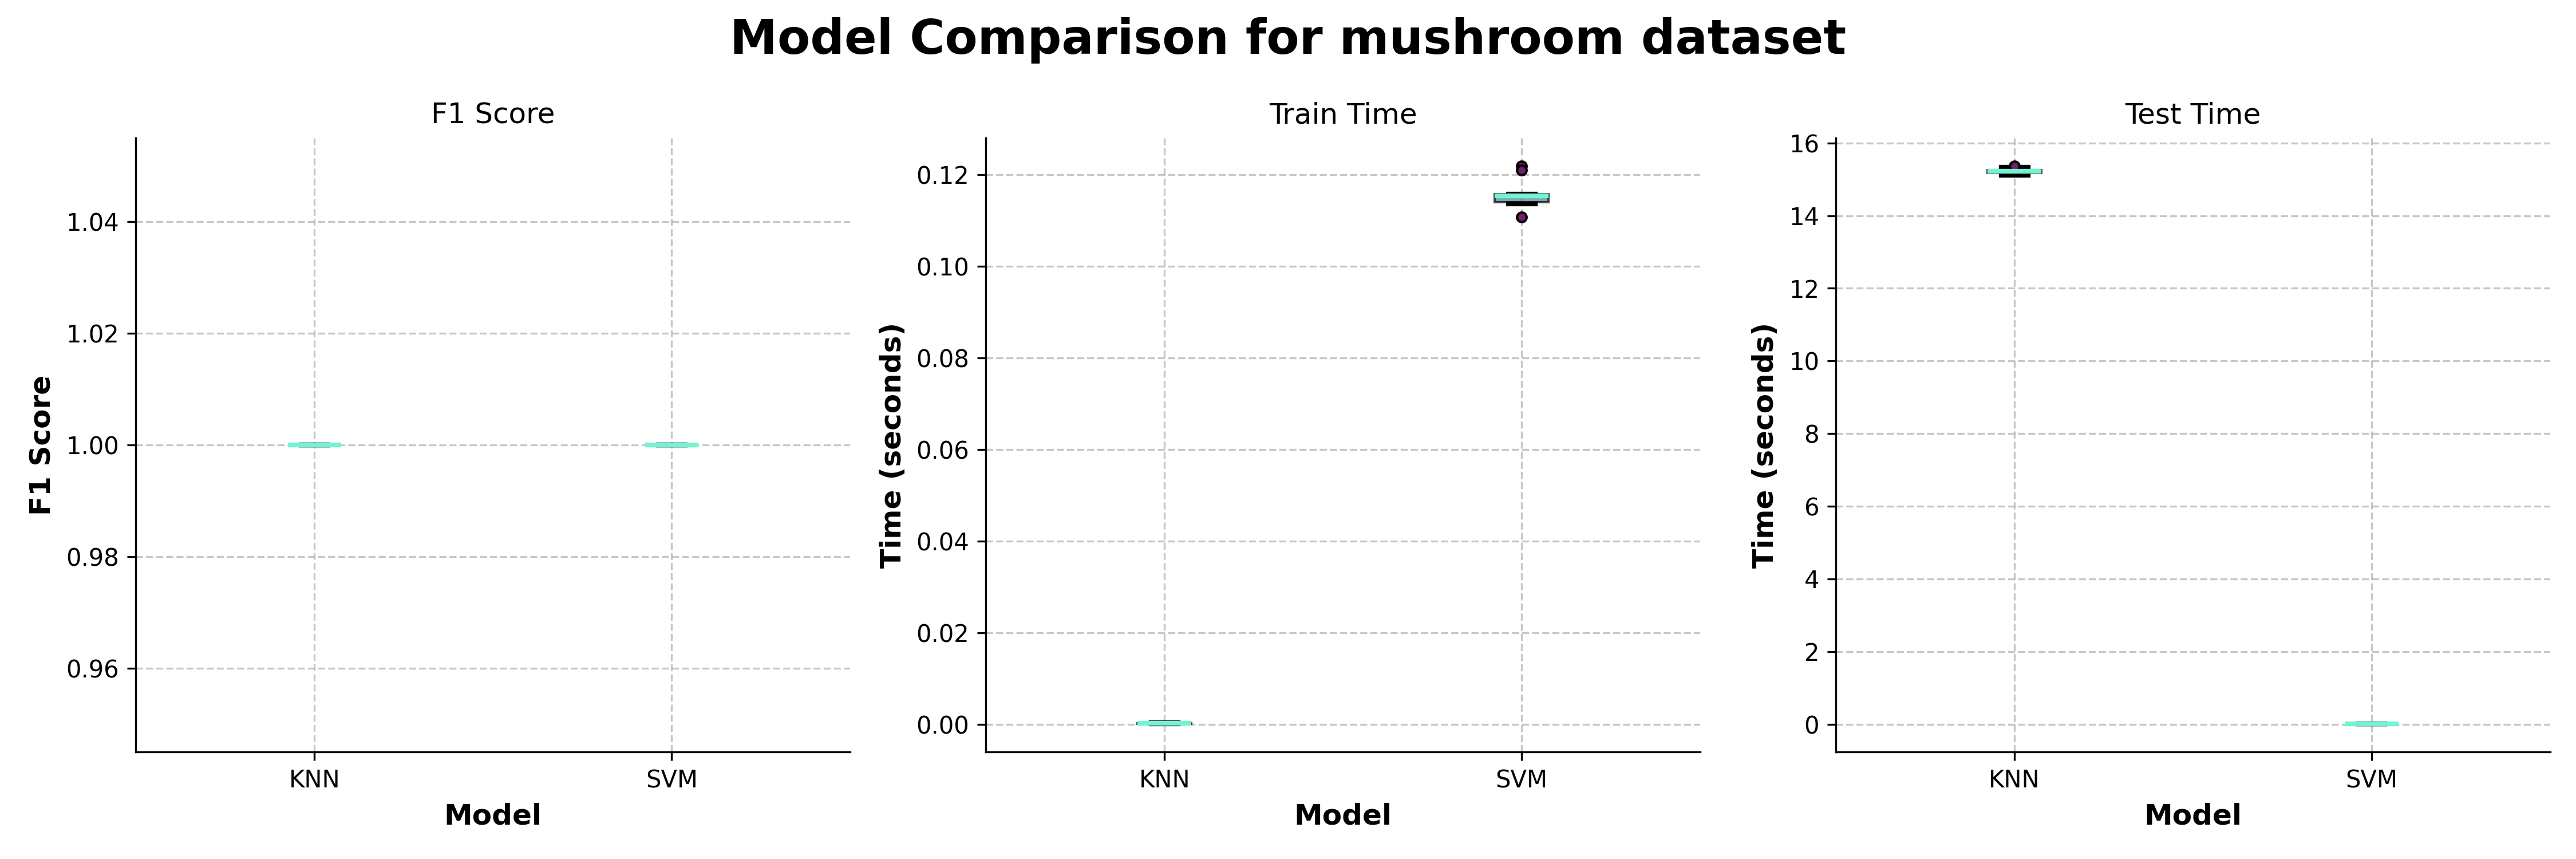
\includegraphics[width=0.9\textwidth]{figures/model_comparison_mushroom.png}
    \caption{SVM and KNN Comparison}
    \label{fig:model_comparison_mushroom}
\end{figure}


\subsubsection*{Hyperparameter Comparison}

For the hepatitis dataset, the configuration using the \textbf{RBF} kernel and $C=7$
achieved outstanding accuracy and F1 scores. However, because of the simple predictability
of the mushroom data, the simple \textbf{Polynomial} kernel performed better when paired with $C=1$.
(See \autoref{tab:svm_results_hepatitis} and \autoref{tab:svm_results_mushroom}).

To compare the performance across model configurations, we employed statistical analysis methods
(see \autoref{sec:statistical-analysis}) to determine whether the various configurations showed
statistically significant differences in performance.

\begin{figure}
    \centering
    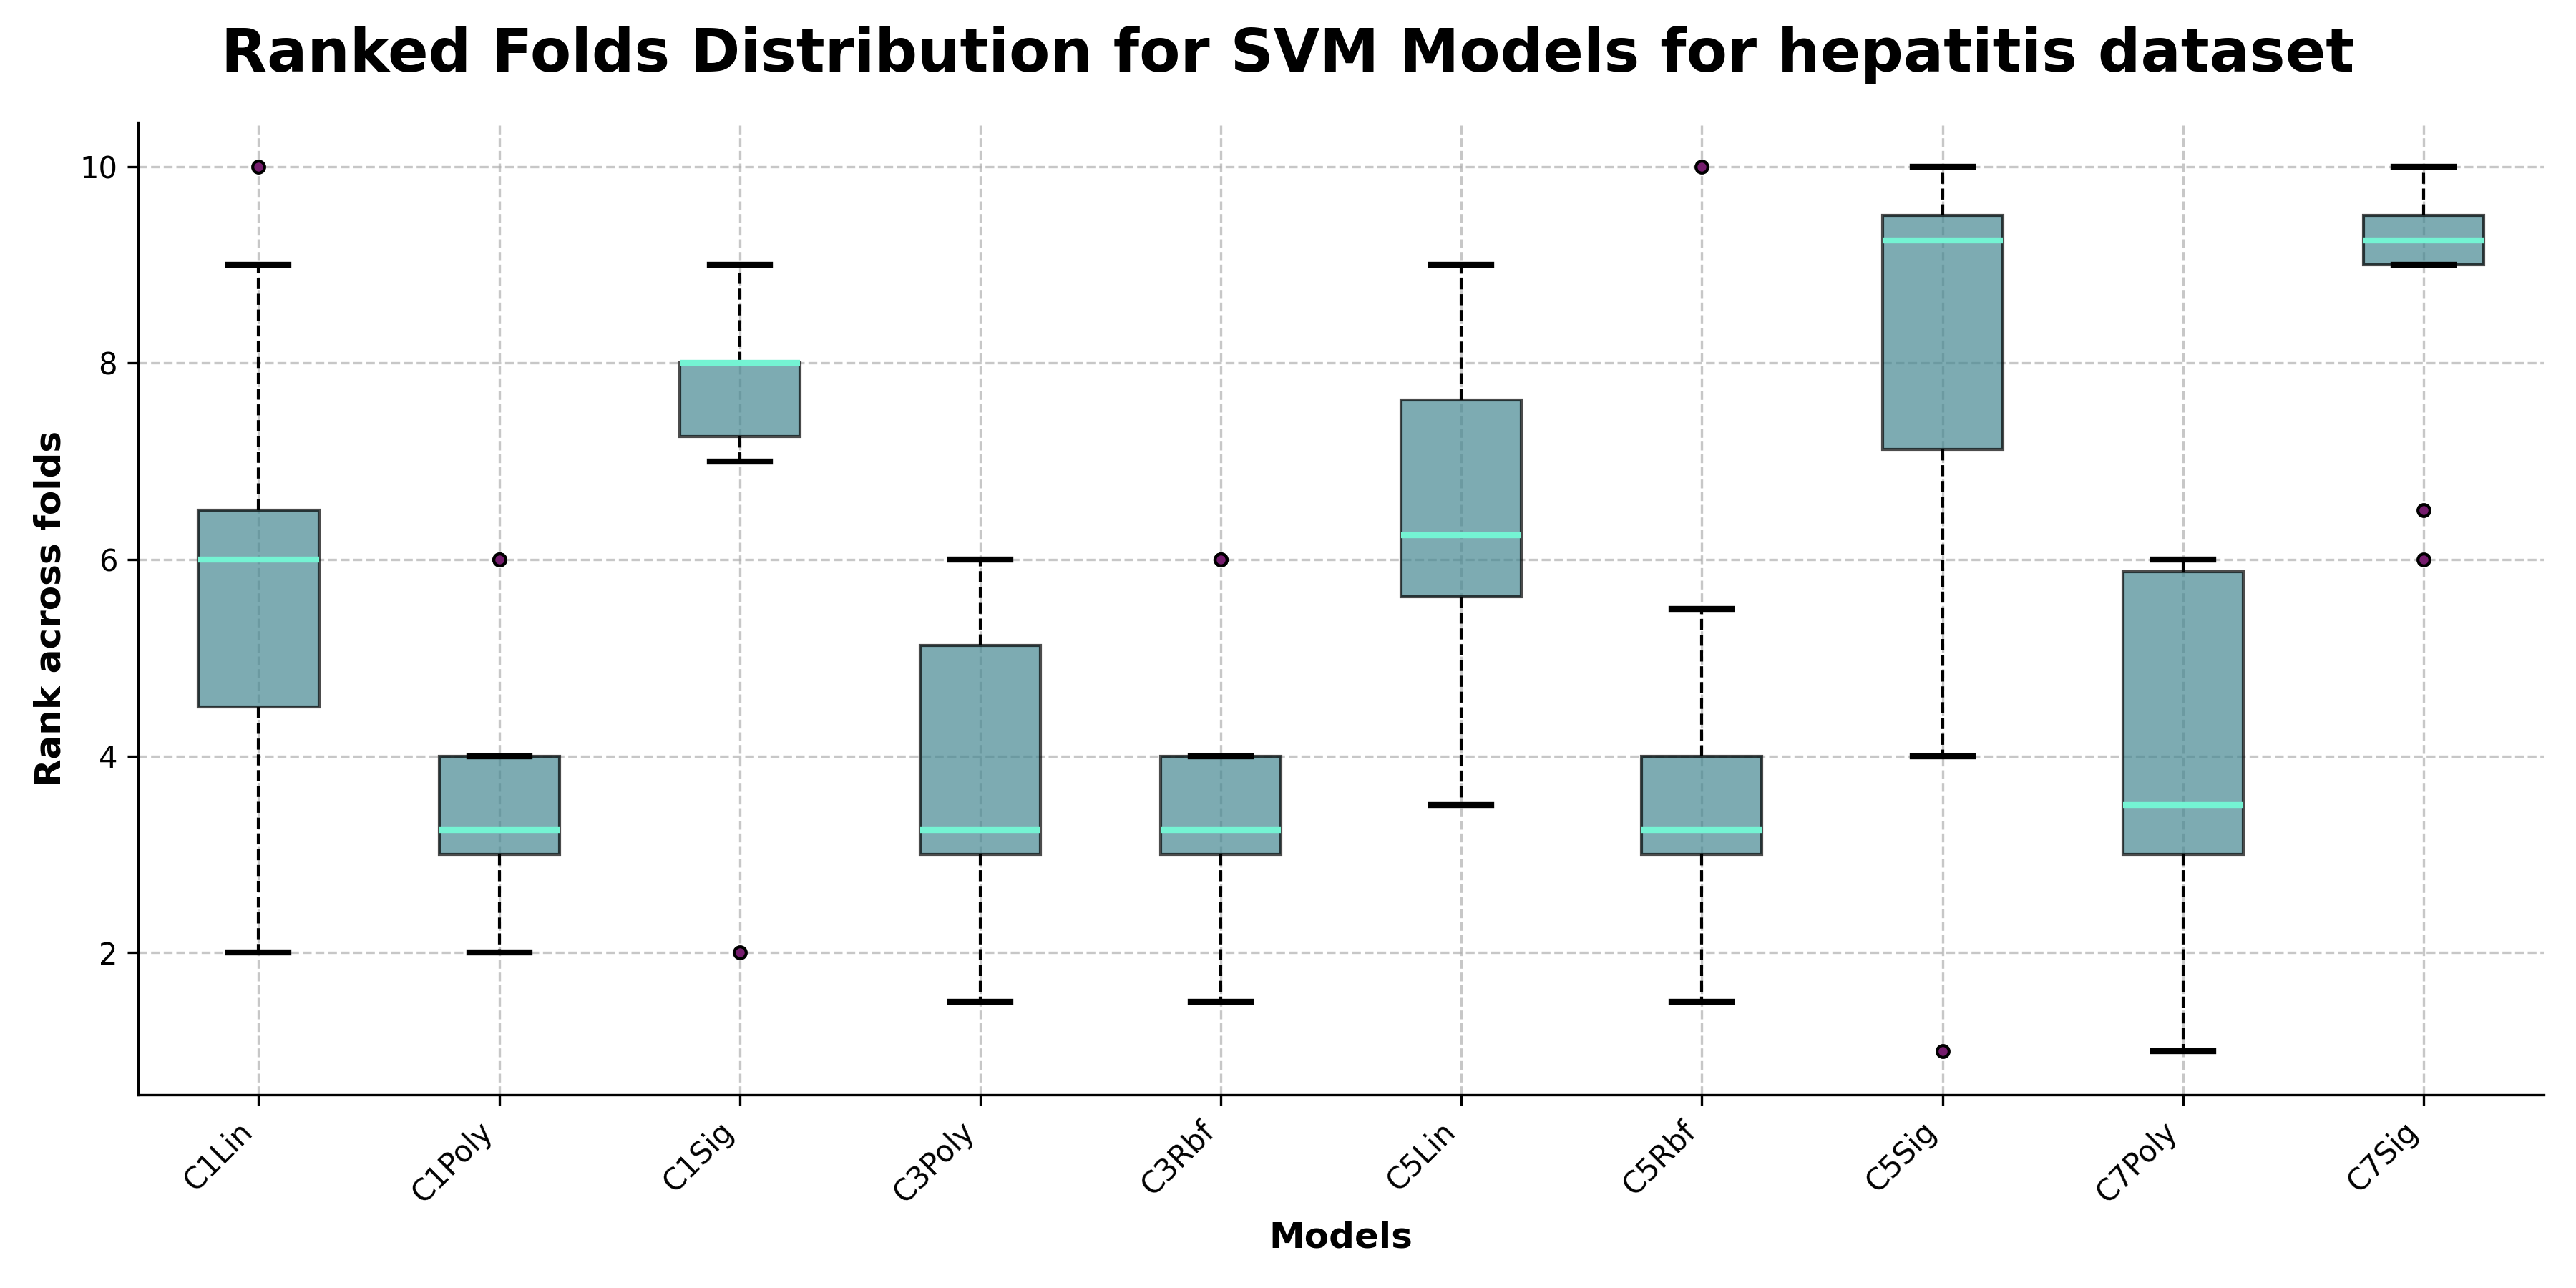
\includegraphics[width=0.9\textwidth]{figures/ranked_folds_SVM_hepatitis.png}
    \caption{SVM Ranked Folds for Hepatitis Dataset}
    \label{fig:ranked_folds_svm_hepatitis}
\end{figure}

\begin{figure}
    \centering
    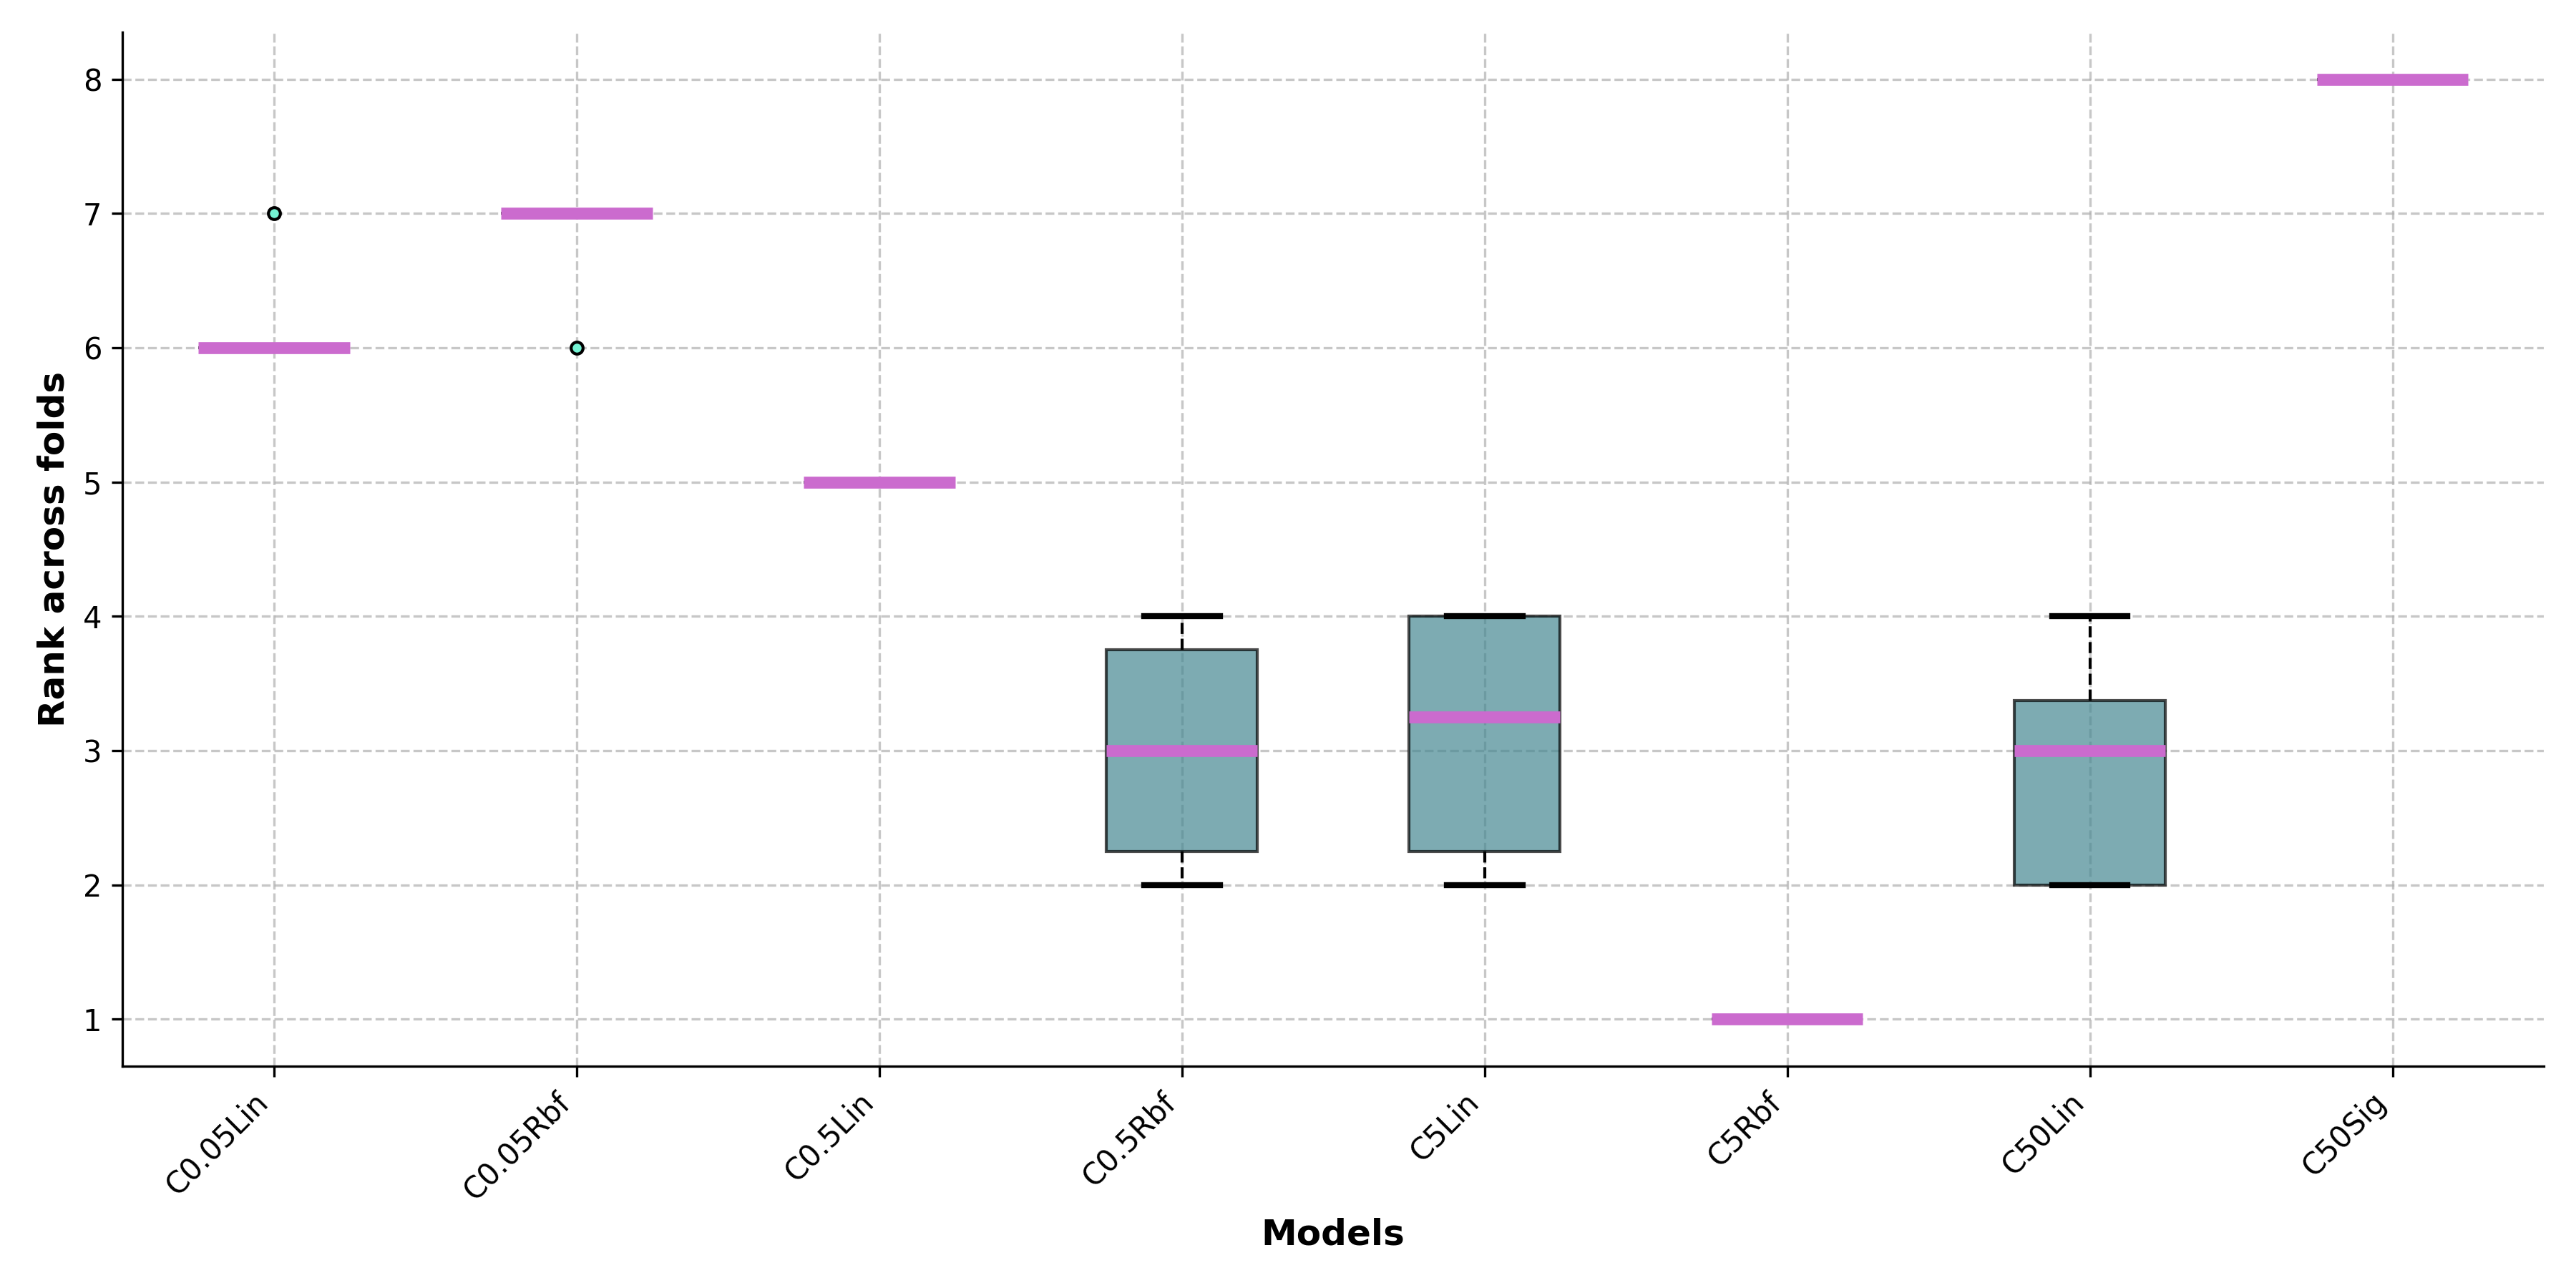
\includegraphics[width=0.9\textwidth]{figures/ranked_folds_SVM_mushroom.png}
    \caption{SVM Ranked Folds for Mushroom Dataset}
    \label{fig:ranked_folds_svm_mushroom}
\end{figure}

As seen in \autoref{fig:ranked_folds_svm_hepatitis} and \autoref{fig:ranked_folds_svm_mushroom},
some models achieved significantly better results than others. By comparing the ranks among each of the 10 folds,
we can check to see if there were any cases in which 1 model always outperformed another.

The mushroom dataset has some especially obvious cases, in which the $C=3$ and $C=5$ RBF models
outperformed all other models across every fold. The $C=5$ RBF model was the best performing model overall.

The hepatitis dataset does not have as extreme of a case, but there are still some models that stand out.
The $C=7$ Sigmoid model was consistently worse than the $C=3$ and $C=5$ RBF models.

\begin{figure}
    \centering
    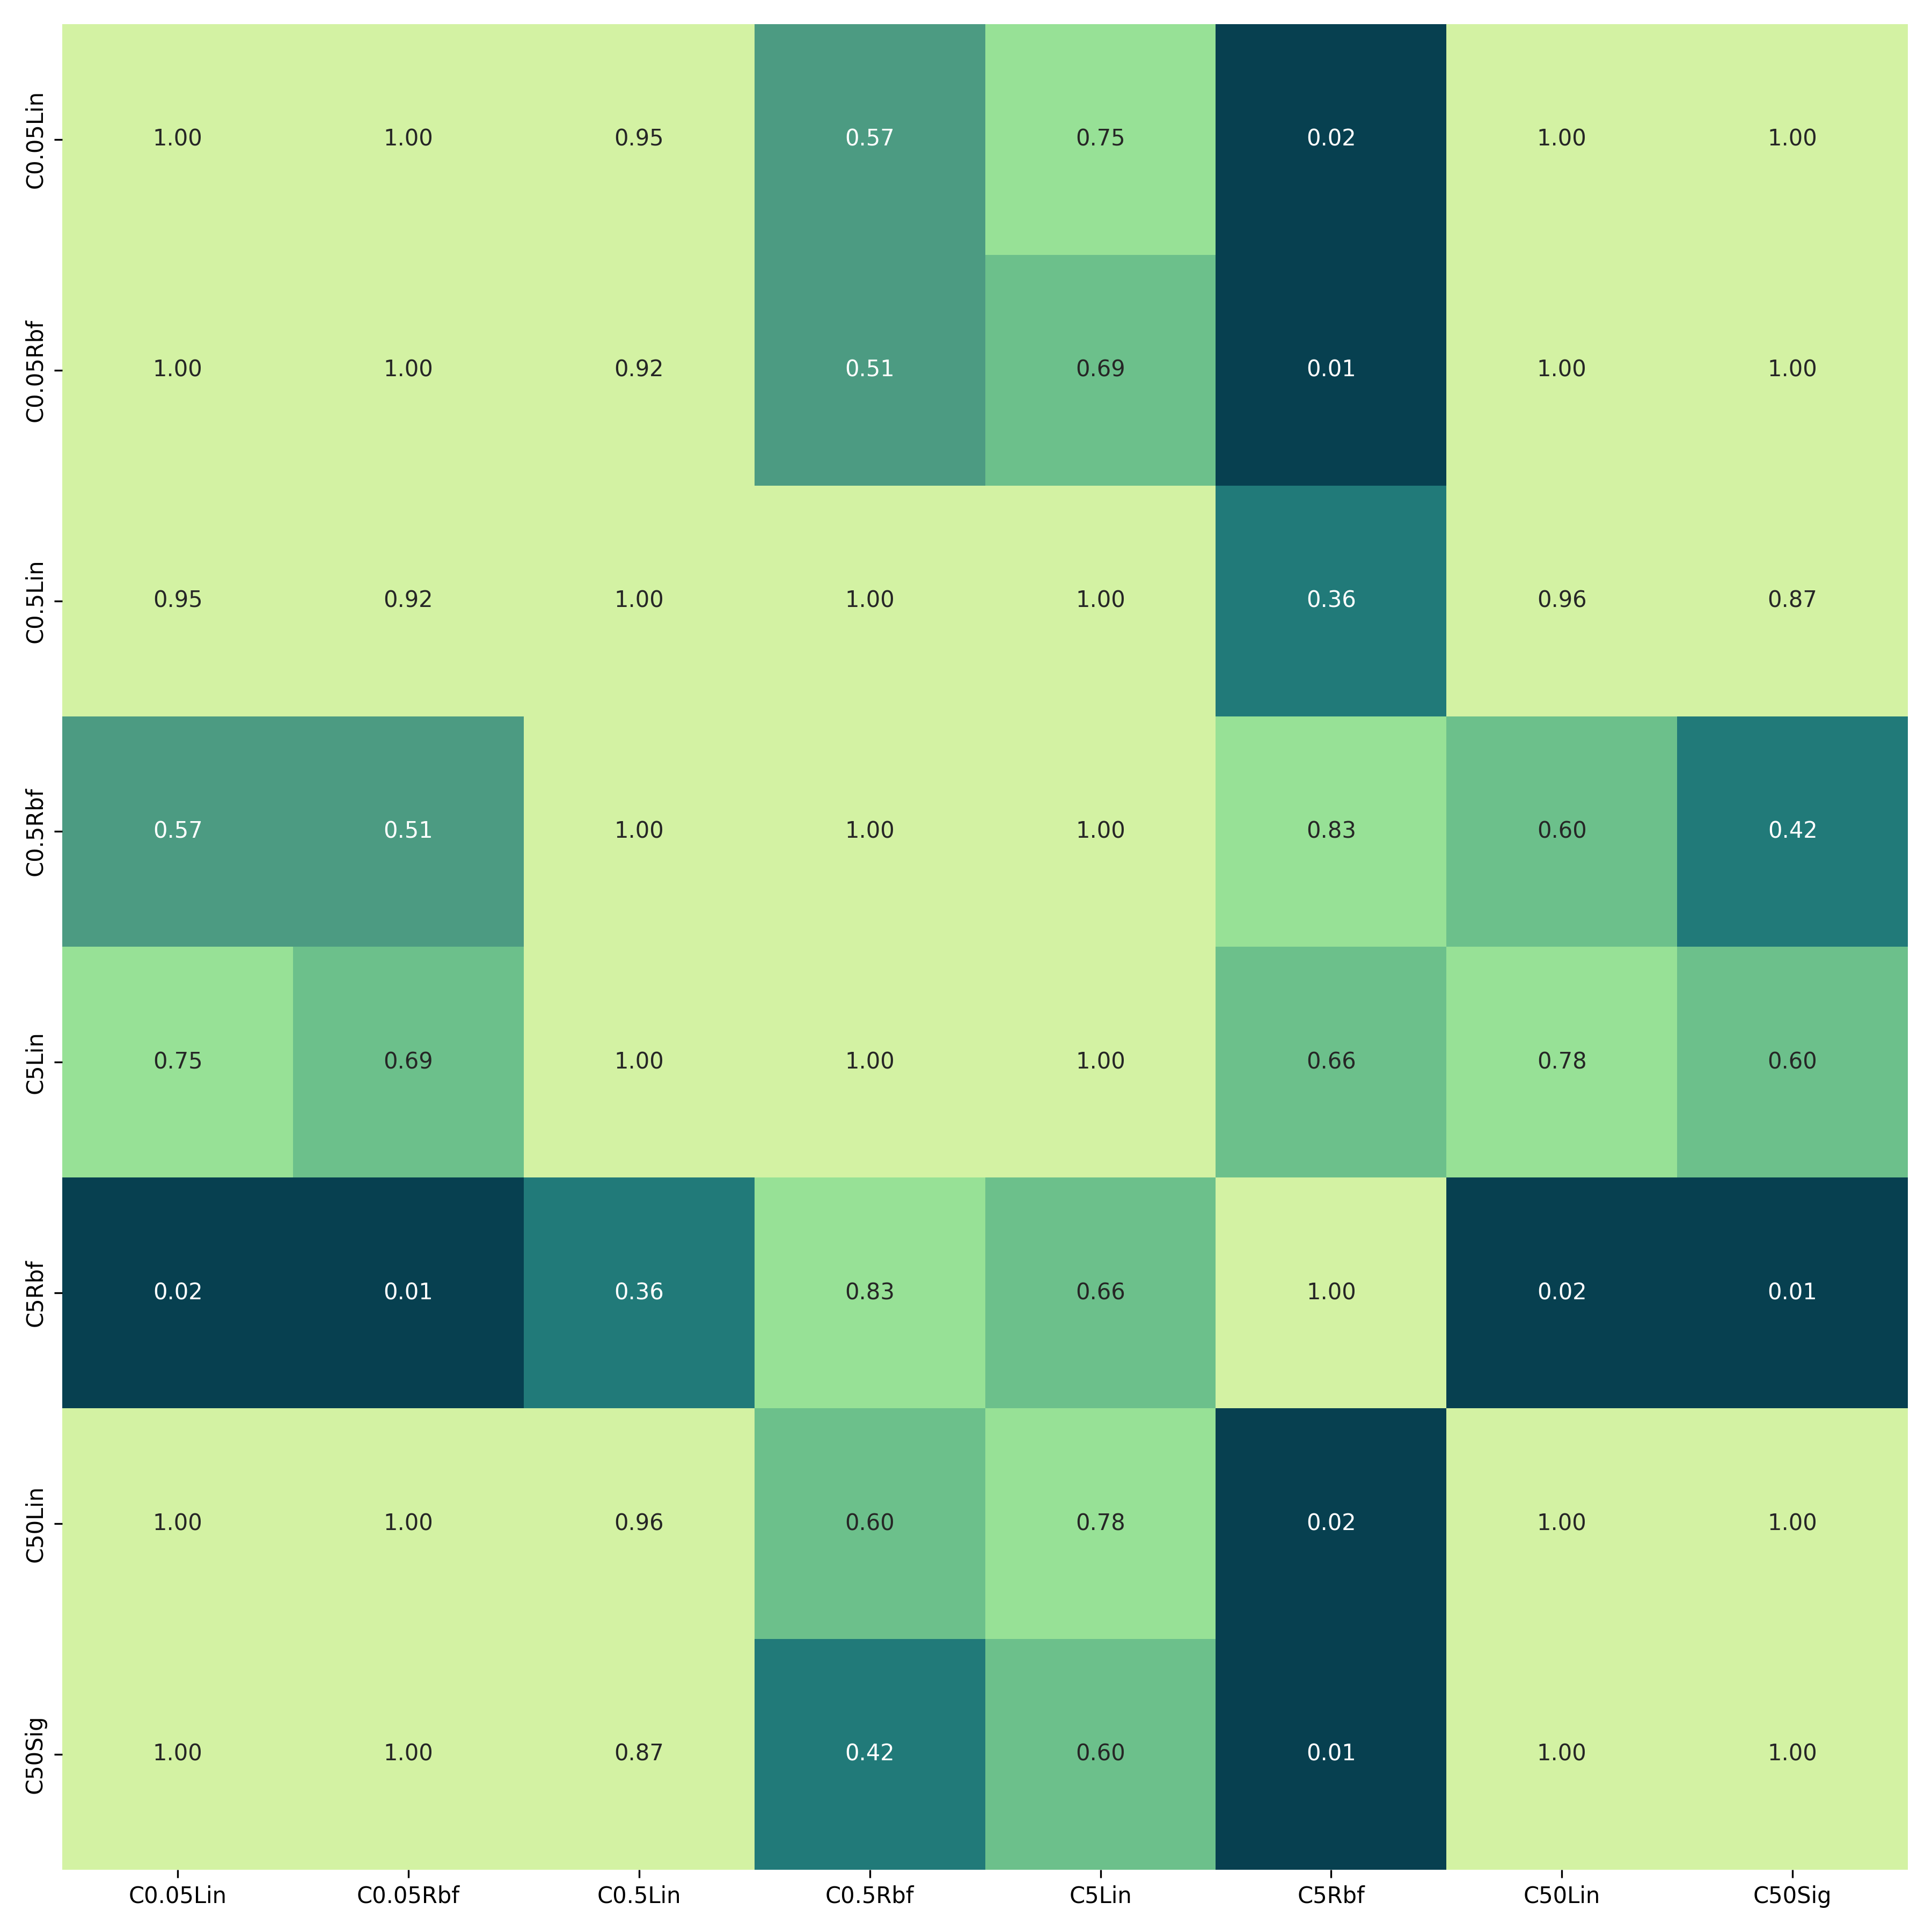
\includegraphics[width=0.4\textwidth]{figures/nemenyi_test_results_SVM_hepatitis.png}
    \caption{Nemenyi Test Results for SVM on Hepatitis Dataset}
    \label{fig:nemenyi_test_results_SVM_hepatitis}
\end{figure}

\begin{figure}
    \centering
    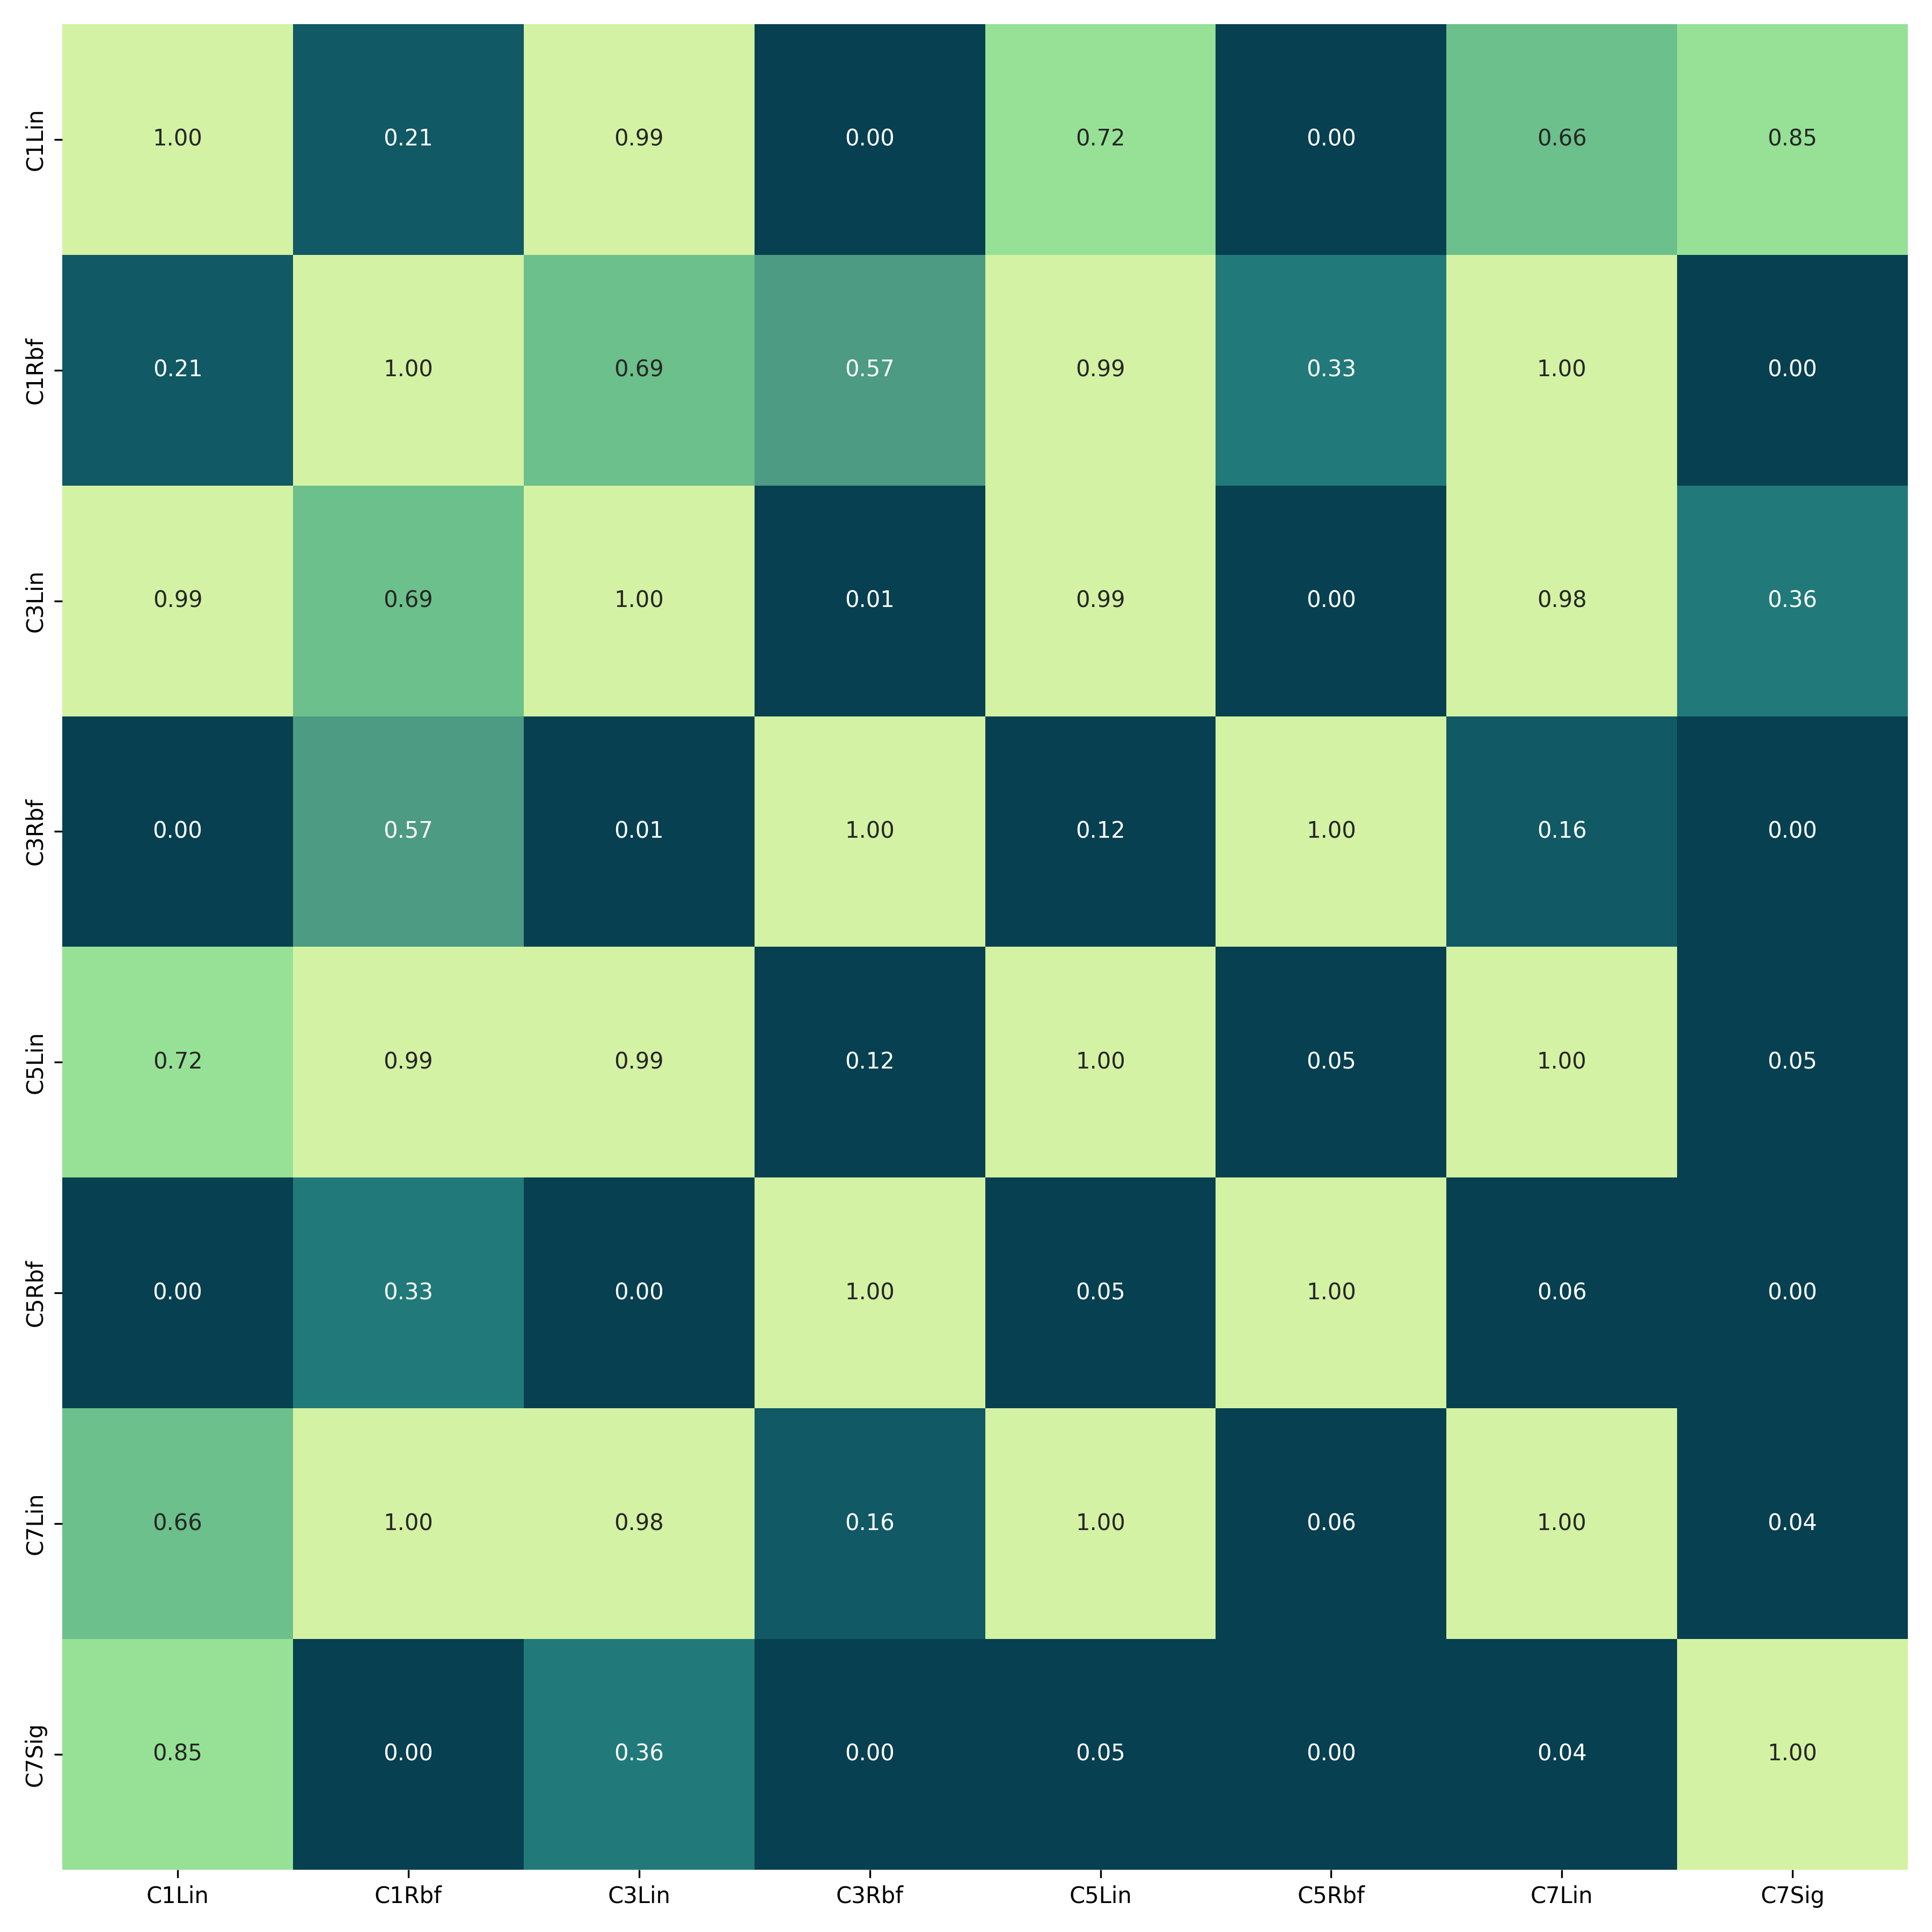
\includegraphics[width=0.4\textwidth]{figures/nemenyi_test_results_SVM_mushroom.png}
    \caption{Nemenyi Test Results for SVM on Mushroom Dataset}
    \label{fig:nemenyi_test_results_SVM_mushroom}
\end{figure}

To identify significant pairs at a glance, we performed the Nemenyi test on all model pairs,
and present them in heatmaps (see \autoref{fig:nemenyi_test_results_SVM_hepatitis} and \autoref{fig:nemenyi_test_results_SVM_mushroom}).
The cells represent the p-values for each pair of models. A value of 0.05 or lower indicates that the models are statistically different
at the 95\% confidence level. The full tables containing the p-values for each pair of significant models are provided in \autoref{tab:svm_significant_pairs_hepatitis} and \autoref{tab:svm_significant_pairs_mushroom}.

\begin{table}
\centering
\caption{Significant Differences in SVM Models}
\label{tab:svm_significant_pairs_hepatitis}
\begin{tabular}{rlrrrrrrrrrrrrrrrrrrrrrrrrrrrrrrrrl}
\toprule
C & Kernel Type & F1 0 & F1 1 & F1 2 & F1 3 & F1 4 & F1 5 & F1 6 & F1 7 & F1 8 & F1 9 & Train Time 0 & Train Time 1 & Train Time 2 & Train Time 3 & Train Time 4 & Train Time 5 & Train Time 6 & Train Time 7 & Train Time 8 & Train Time 9 & Test Time 0 & Test Time 1 & Test Time 2 & Test Time 3 & Test Time 4 & Test Time 5 & Test Time 6 & Test Time 7 & Test Time 8 & Test Time 9 & Mean F1 Score & Std F1 Score & Model Label \\
\midrule
3 & rbf & 0.857 & 0.966 & 1.000 & 1.000 & 1.000 & 1.000 & 0.909 & 1.000 & 0.957 & 1.000 & 0.001 & 0.001 & 0.001 & 0.001 & 0.001 & 0.001 & 0.001 & 0.001 & 0.001 & 0.001 & 0.000 & 0.000 & 0.000 & 0.000 & 0.000 & 0.000 & 0.000 & 0.000 & 0.000 & 0.000 & 0.969 & 0.049 & C3Rbf \\
5 & rbf & 0.828 & 0.966 & 1.000 & 1.000 & 0.960 & 1.000 & 0.957 & 1.000 & 1.000 & 1.000 & 0.001 & 0.001 & 0.001 & 0.001 & 0.001 & 0.001 & 0.001 & 0.001 & 0.001 & 0.001 & 0.000 & 0.000 & 0.000 & 0.000 & 0.000 & 0.000 & 0.000 & 0.000 & 0.000 & 0.000 & 0.971 & 0.054 & C5Rbf \\
7 & sigmoid & 0.857 & 0.667 & 0.815 & 0.909 & 0.846 & 0.846 & 0.846 & 0.750 & 0.909 & 0.846 & 0.001 & 0.001 & 0.001 & 0.001 & 0.001 & 0.001 & 0.001 & 0.001 & 0.001 & 0.001 & 0.000 & 0.000 & 0.000 & 0.001 & 0.000 & 0.000 & 0.000 & 0.000 & 0.000 & 0.000 & 0.829 & 0.073 & C7Sig \\
\bottomrule
\end{tabular}
\end{table}

\begin{table}
\centering
\caption{Significant Differences in SVM Models}
\label{tab:svm_significant_pairs_mushroom}
\begin{tabular}{rlrrrrrrrrrrrrrrrrrrrrrrrrrrrrrrrrrl}
\toprule
C & kernel_type & f1_0 & f1_1 & f1_2 & f1_3 & f1_4 & f1_5 & f1_6 & f1_7 & f1_8 & f1_9 & train_time_0 & train_time_1 & train_time_2 & train_time_3 & train_time_4 & train_time_5 & train_time_6 & train_time_7 & train_time_8 & train_time_9 & test_time_0 & test_time_1 & test_time_2 & test_time_3 & test_time_4 & test_time_5 & test_time_6 & test_time_7 & test_time_8 & test_time_9 & mean_f1 & mean_train_time & mean_test_time & model_label \\
\midrule
1 & linear & 0.983 & 0.971 & 0.976 & 0.968 & 0.982 & 0.975 & 0.964 & 0.978 & 0.973 & 0.976 & 0.556 & 0.793 & 0.566 & 0.486 & 0.579 & 0.412 & 0.631 & 0.548 & 0.694 & 0.514 & 0.015 & 0.013 & 0.014 & 0.017 & 0.014 & 0.014 & 0.013 & 0.015 & 0.013 & 0.014 & 0.975 & 0.578 & 0.014 & C1Lin \\
1 & rbf & 0.983 & 0.991 & 0.982 & 0.992 & 0.991 & 0.988 & 0.988 & 0.996 & 0.990 & 0.988 & 0.180 & 0.178 & 0.178 & 0.180 & 0.178 & 0.176 & 0.176 & 0.179 & 0.178 & 0.176 & 0.030 & 0.030 & 0.030 & 0.030 & 0.030 & 0.030 & 0.030 & 0.030 & 0.031 & 0.030 & 0.989 & 0.178 & 0.030 & C1Rbf \\
3 & linear & 0.989 & 0.978 & 0.981 & 0.971 & 0.985 & 0.975 & 0.978 & 0.981 & 0.986 & 0.972 & 0.724 & 0.682 & 0.690 & 0.993 & 0.759 & 1.305 & 0.662 & 0.961 & 0.734 & 0.810 & 0.012 & 0.012 & 0.012 & 0.012 & 0.011 & 0.010 & 0.013 & 0.013 & 0.012 & 0.012 & 0.980 & 0.832 & 0.012 & C3Lin \\
3 & rbf & 0.996 & 1.000 & 1.000 & 1.000 & 0.999 & 0.997 & 1.000 & 1.000 & 0.997 & 0.997 & 0.121 & 0.121 & 0.120 & 0.124 & 0.121 & 0.122 & 0.122 & 0.119 & 0.121 & 0.120 & 0.018 & 0.018 & 0.018 & 0.018 & 0.018 & 0.018 & 0.018 & 0.018 & 0.018 & 0.018 & 0.999 & 0.121 & 0.018 & C3Rbf \\
5 & linear & 0.977 & 0.985 & 0.985 & 0.972 & 0.994 & 0.975 & 0.987 & 0.987 & 0.992 & 0.973 & 1.316 & 1.133 & 1.250 & 1.178 & 1.111 & 1.675 & 1.068 & 1.013 & 1.131 & 0.975 & 0.013 & 0.013 & 0.012 & 0.011 & 0.013 & 0.012 & 0.015 & 0.012 & 0.013 & 0.014 & 0.983 & 1.185 & 0.013 & C5Lin \\
5 & rbf & 0.999 & 1.000 & 1.000 & 1.000 & 1.000 & 1.000 & 1.000 & 1.000 & 0.997 & 1.000 & 0.101 & 0.100 & 0.098 & 0.103 & 0.104 & 0.100 & 0.099 & 0.101 & 0.102 & 0.102 & 0.014 & 0.014 & 0.013 & 0.014 & 0.014 & 0.014 & 0.014 & 0.014 & 0.014 & 0.014 & 1.000 & 0.101 & 0.014 & C5Rbf \\
7 & linear & 0.980 & 0.986 & 0.990 & 0.972 & 0.986 & 0.975 & 0.989 & 0.976 & 0.991 & 0.984 & 1.351 & 1.625 & 1.357 & 1.318 & 1.506 & 1.418 & 2.815 & 1.468 & 1.493 & 1.878 & 0.016 & 0.014 & 0.015 & 0.015 & 0.016 & 0.016 & 0.014 & 0.015 & 0.016 & 0.016 & 0.983 & 1.623 & 0.015 & C7Lin \\
7 & sigmoid & 0.390 & 0.459 & 0.708 & 0.391 & 0.479 & 0.428 & 0.432 & 0.368 & 0.358 & 0.346 & 0.807 & 0.804 & 0.478 & 0.800 & 0.807 & 0.805 & 0.801 & 0.802 & 0.809 & 0.806 & 0.077 & 0.078 & 0.048 & 0.077 & 0.078 & 0.077 & 0.077 & 0.077 & 0.077 & 0.077 & 0.436 & 0.772 & 0.075 & C7Sig \\
\bottomrule
\end{tabular}
\end{table}


\begin{figure}
    \centering
    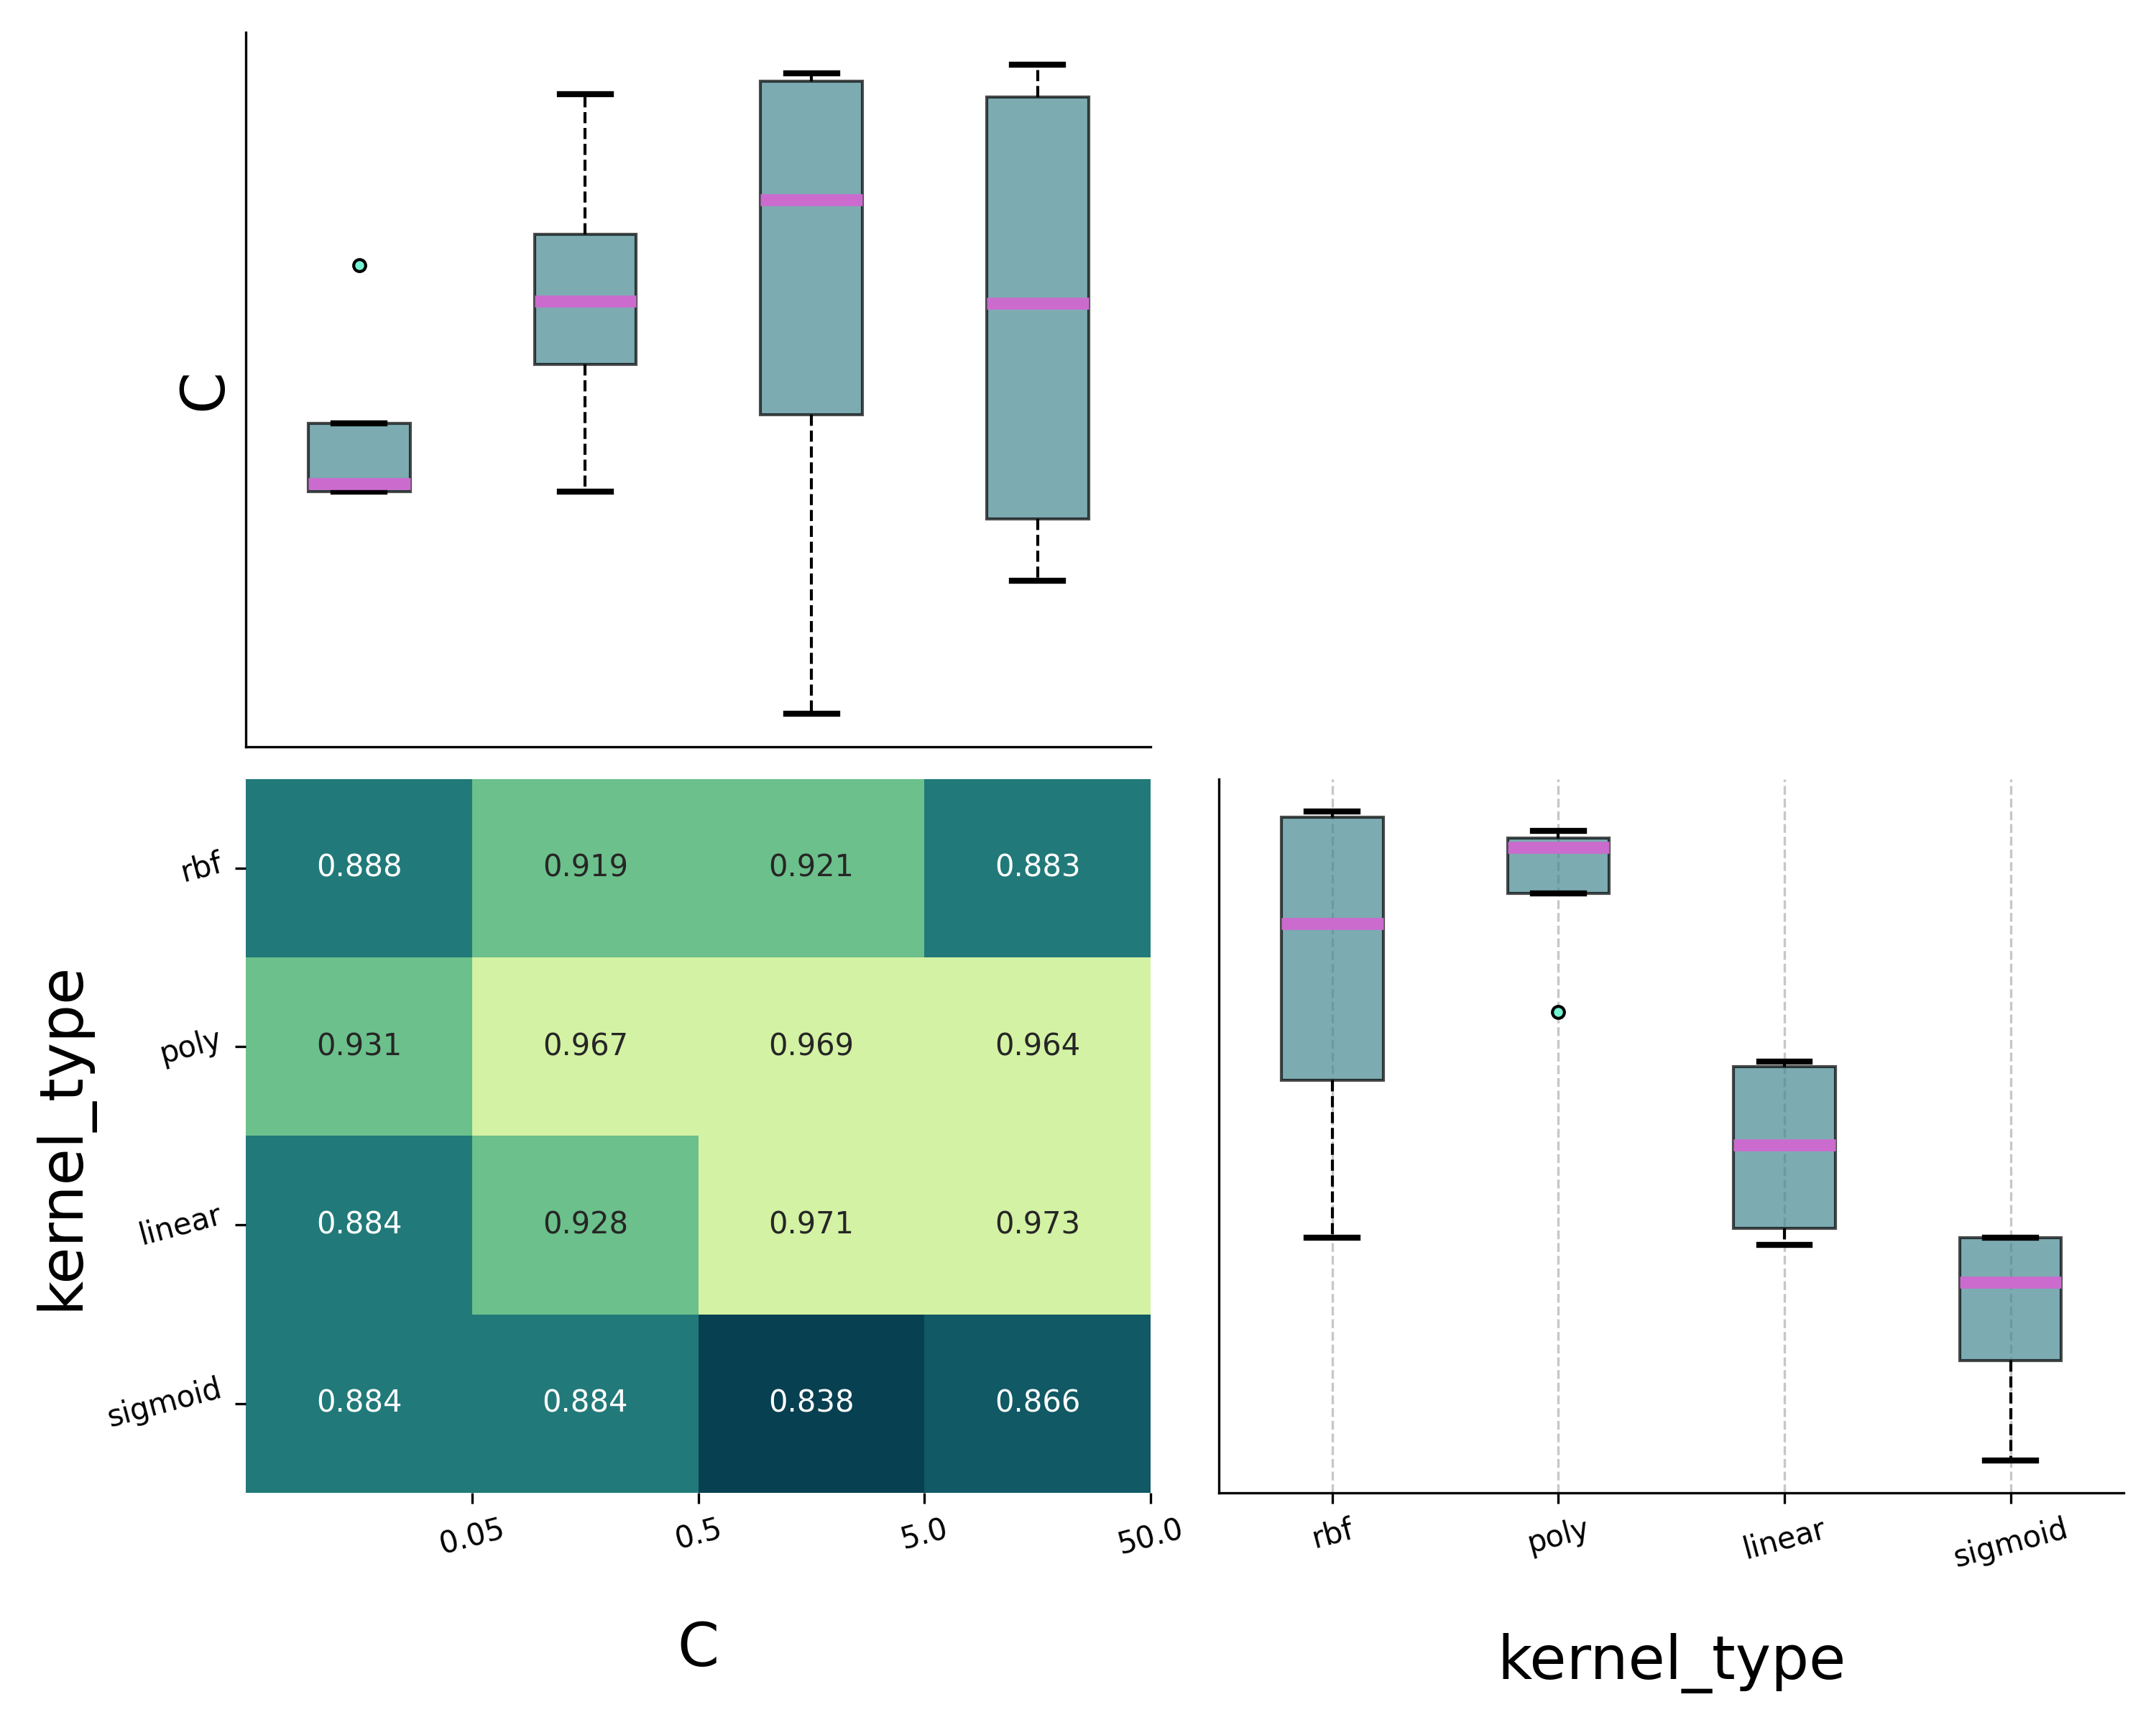
\includegraphics[width=0.4\textwidth]{figures/interaction_effects_SVM_hepatitis.png}
    \caption{Nemenyi Test Results for SVM on Mushroom Dataset}
    \label{fig:interaction_effects_SVM_hepatitis}
\end{figure}

To further analyze the hyperparameters we plotted the effects of each hyperparameter on the F1 score.

